\noindent 
Thus, the goal is to demonstrate that the minimal assembly language 
presented is powerful enough to express a calculation that allows the 
assembly of two-dimensional blocks using an instruction manual. 
\medskip

\noindent 
There are two formats for the instruction manual that the assembler 
program can interpret in language $L'$: 
\begin{enumerate} 
  \item \emph{First format} 
    \begin{itemize} 
      \item \texttt{1st byte}: width (4 bits) and height (4 bits) of 
      the piece. 
      \item \texttt{2nd byte}: horizontal (4 bits) and vertical (4 
        bits) offset of the piece. 
      \item \texttt{3rd byte}: color of the piece. 
    \end{itemize} 
    For example, 
    $\texttt{MEM} {:=} [0x11, 0x22, 0x07, 0x21, 0x10, 0x06]$ can be 
    translated as: 
    \begin{enumerate} 
      \item[1.] Place a $1 \times 1$ piece with a displacement of 
        $(2, 2)$ and color $0x07$. 
      \item[2.] Place a $2 \times 1$ piece with a displacement of 
        $(1, 0)$ and color $0x06$. 
    \end{enumerate} 
  \item \emph{Second format} 
    \begin{itemize} 
      \item \texttt{1st byte}: width of the piece. 
      \item \texttt{2nd byte}: height of the piece. 
      \item \texttt{3rd byte}: horizontal offset of the piece. 
      \item \texttt{4th byte}: vertical offset of the piece. 
      \item \texttt{5th byte}: color of the piece. 
    \end{itemize} 
    For example, $\texttt{MEM} {:=} [0x01, 0x01, 0x02, 0x02, 0x07, 
    0x02, 0x01, 0x01, 0x00, 0x06]$ can be translated as: 
    \begin{enumerate} 
      \item[1.] Place a $1 \times 1$ piece with a displacement of 
        $(2, 2)$ and color $0x07$. 
      \item[2.] Place a $2 \times 1$ piece with a displacement of 
        $(1, 0)$ and color $0x06$. 
    \end{enumerate}
\end{enumerate} 
The assembler program must be able to read an instruction manual 
(found in MEM) in one of the two formats and assemble the blocks to 
form a two-dimensional construction. 
\medskip

\noindent 
The positioning follows a cumulative logic: initially at $(0, 0)$, the 
top-left corner, each piece is placed relative to the previous one. 
Its anchor is set at its top-left corner. To make this decidable, the 
size of the grid used to place the pieces (\texttt{MAP}) is set to 
$8 \times 8$. When a displacement causes an overflow of the grid, the 
program must reposition its anchor to position $0$ in that dimension. 
That is, if a piece is displaced by $(4, 3)$ and we are at position 
$(5, 6)$, the piece will be placed at position $((5 + 4) \mod 8, 
(6 + 3) \mod 8) = (1, 1)$. This same logic applies when part of the 
piece exceeds the grid. The final anchor point after placing a piece 
is given by the following formula: $((p_{ix} + w + dx) \mod 8, (p_{iy} 
+ h + dy - 1) \mod 8)$ where $p_{ix}$ and $p_{iy}$ are the coordinates 
of the top-left corner of the initial anchor point, $w$ and $h$ are 
the width and height of the piece respectively, and $dx$ and $dy$ are 
the horizontal and vertical displacements of the piece. 
\medskip

\noindent 
The illustration below shows the evolution of the grid after placing 
the pieces for the memory \\ $\texttt{MEM} {:=} [0x11, 0x22, 0x07, 
0x21, 0x00, 0x06]$ (first format): 
\medskip

\begin{minipage}{0.2\textwidth}
{\scriptsize Initially : }\\
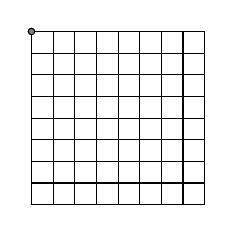
\begin{tikzpicture}[scale=0.275]
  \foreach \x in {0, 1, ..., 7} {
    \foreach \y in {0, 1, ..., 7} {
      \draw[fill=white] (\x, \y) rectangle (\x + 1, \y + 1);
    }
  }

  \draw[fill=gray] (0, 8) circle (0.15);
\end{tikzpicture}
\end{minipage}
\begin{minipage}{0.2\textwidth}
{\scriptsize After the first piece :} \\
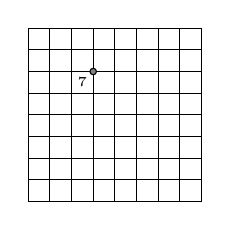
\begin{tikzpicture}[scale=0.275]
  \foreach \x in {0, 1, ..., 7} {
    \foreach \y in {0, 1, ..., 7} {
      \draw[fill=white] (\x, \y) rectangle (\x + 1, \y + 1);
    }
  }

  \draw[fill=gray] (3, 6) circle (0.15);
  \node[font=\tiny] at (2.5, 5.5) {7};
\end{tikzpicture}
\end{minipage}
\begin{minipage}{0.33\textwidth}
  {\scriptsize After the second piece :} \\
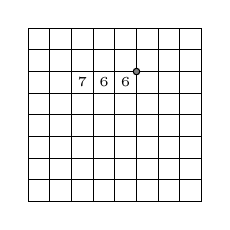
\begin{tikzpicture}[scale=0.275]
  \foreach \x in {0, 1, ..., 7} {
    \foreach \y in {0, 1, ..., 7} {
      \draw[fill=white] (\x, \y) rectangle (\x + 1, \y + 1);
    }
  }

  \draw[fill=gray] (5, 6) circle (0.15);
  \node[font=\tiny] at (2.5, 5.5) {7};
  \node[font=\tiny] at (3.5, 5.5) {6};
  \node[font=\tiny] at (4.5, 5.5) {6};
\end{tikzpicture}
\end{minipage}
\medskip

\noindent 
The goal is therefore, in the first phase, to translate an instruction 
manual into a construction in the grid \texttt{MAP}. In the second 
phase, we conjecture that there are several arrangements of 
instructions that allow the creation of a minimal assembler program 
$L'$ capable of performing this task. The program should therefore be 
optimized to use as few cycles as possible before completing 
construction.
